\documentclass[a4paper,12pt]{report}
\usepackage{float, amsmath, bm, graphicx, numprint, multicol, caption}

\begin{document}

\setlength{\abovedisplayskip}{6pt}
\setlength{\belowdisplayskip}{8pt}
\setlength{\abovedisplayshortskip}{2pt}
\setlength{\belowdisplayshortskip}{8pt}

\title{Project 5 Report}
\author{Dylan Callaway}
\date{Engineering 150 \\ Fall 2019}
\maketitle

\pagenumbering{roman}
\tableofcontents
\newpage
\pagenumbering{arabic}

\newenvironment{nscenter}
 {\setlength{\topsep}{0ex}\trivlist\item\relax\centering}
 {\endtrivlist}

\section{Introduction}
This project models the development of a new material comprised of two other constituent materials. The goal is to use the model in order to select constituent materials, as well as the ratio at which they are mixed, such that desired final material properties are achieved.

The model of the new material is constructed by using the bounds proposed by Hashin and Shtrikman (HS) in their 1963 paper.\footnote{Hashin, Z, and Shtrikman, S, 1963, A variational approach to the elastic behavior of multiphase minerals. Journal of the Mechanics and Physics of Solids} These bounds are the upper and lower limit on the overall properties of the new material, which is assumed to be isotropic, as a function of the properties of constituent isotropic materials.

The properties of interest in this case are the bulk modulus, shear modulus, electrical conductivity, and thermal conductivity; denoted $\kappa$, $\mu$, $\sigma_e$, and $K$, respectively. The effective properties of the new material are denoted with the $^*$ superscript, and the properties of the constituent materials are denoted with either the $_1$ or $_2$ subscripts.

This paper will develop the necessary physical background for the modeling of the materials, outline the specific methods used in the implementation of the governing physics equations, and finally discuss the resulting material properties achieved and how various algorithmic changes affected the outcomes.

\section{Background and Theory}
Using the HS bounds for the properties of interest in this project produces the following equations for the bulk modulus, shear modulus, electrical conductivity, and thermal conductivity as functions of the volume fraction of each constituent material, $v_2$.
\begin{equation}
\kappa_1 + \frac{v_2}{ \frac{1}{\kappa_2-\kappa_1} + \frac{3(1-v_2)}{3\kappa_1 + 4\mu_1} } \leq \kappa^* \leq \kappa_2 + \frac{1-v_2}{ \frac{1}{\kappa_1-\kappa_2} + \frac{3v_2}{3\kappa_2 + 4\mu_2}}
\end{equation}

\begin{equation}
\mu_1 + \frac{v_2}{\frac{1}{\mu_2 - \mu_1} + \frac{6(1-v_2)(\kappa_1 + 2\mu_1)}{5\mu_1(3\kappa_1 + 4\mu_1)}} \leq \mu^* \leq \mu_2 + \frac{1-v_2}{\frac{1}{\mu_1-\mu_2} + \frac{6v_2(\kappa_2+2\mu_2)}{5\mu_2(3\kappa_2+4\mu_2)}}
\end{equation}

\begin{equation}
\sigma_{e,1} + \frac{v_2}{\frac{1}{\sigma_{e,2}-\sigma_{e,1}} + \frac{1-v_2}{3\sigma_{e,1}}} \leq \sigma^*_e \leq \sigma_{e,2} + \frac{1-v_2}{\frac{1}{\sigma_{e,1} - \sigma_{e,2}} + \frac{v_2}{3\sigma_{e,2}}}
\end{equation}

\begin{equation}
K_1 + \frac{v_2}{\frac{1}{K_2-K_1} + \frac{1-v_2}{3K_1}} \leq K^* \leq K_2 + \frac{1-v_2}{\frac{1}{K_2-K_2} + \frac{v_2}{3K_2}}
\end{equation}

When used to compare with the desired material properties, the average of the upper and lower HS bound is taken for each property according to:
\begin{equation}
y^* \approx \phi y^{*,-} + (1-\phi)y^{*,+}
\end{equation}
where $\phi = 0.5$, $y$ is some material property, and the $^-$ and $^+$ superscripts denote the lower and upper bound, respectively.



\section{Procedure and Methods}


\section{Results and Discussion}

\begin{figure}[H]
\begin{nscenter}
  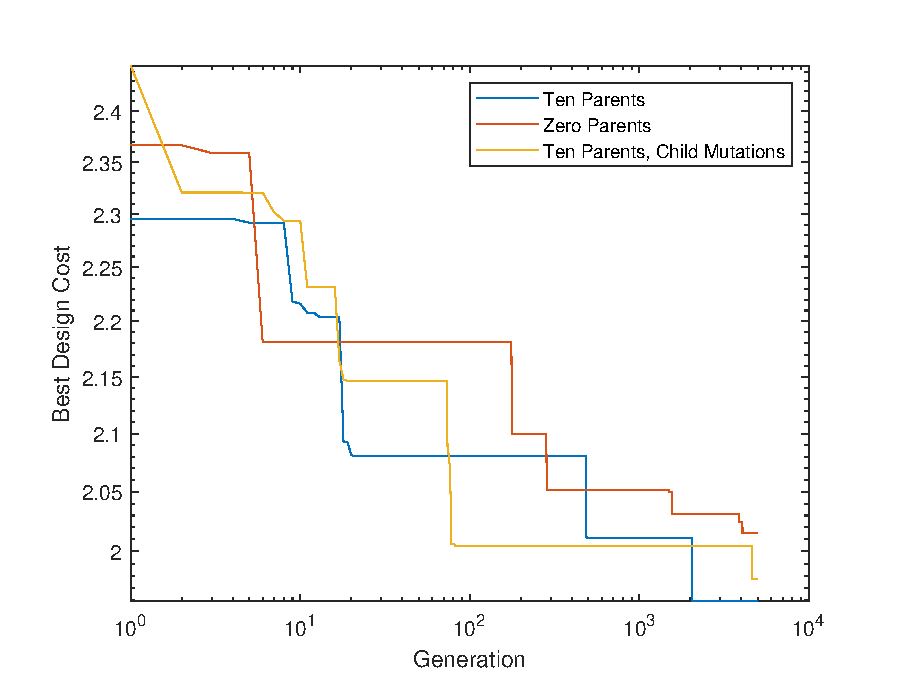
\includegraphics[width=0.75\linewidth]{2-1.eps}
  \caption{Cost of best design vs. generation for various GA types.}
  \end{nscenter}
\end{figure}

\begin{figure}[H]
\begin{nscenter}
  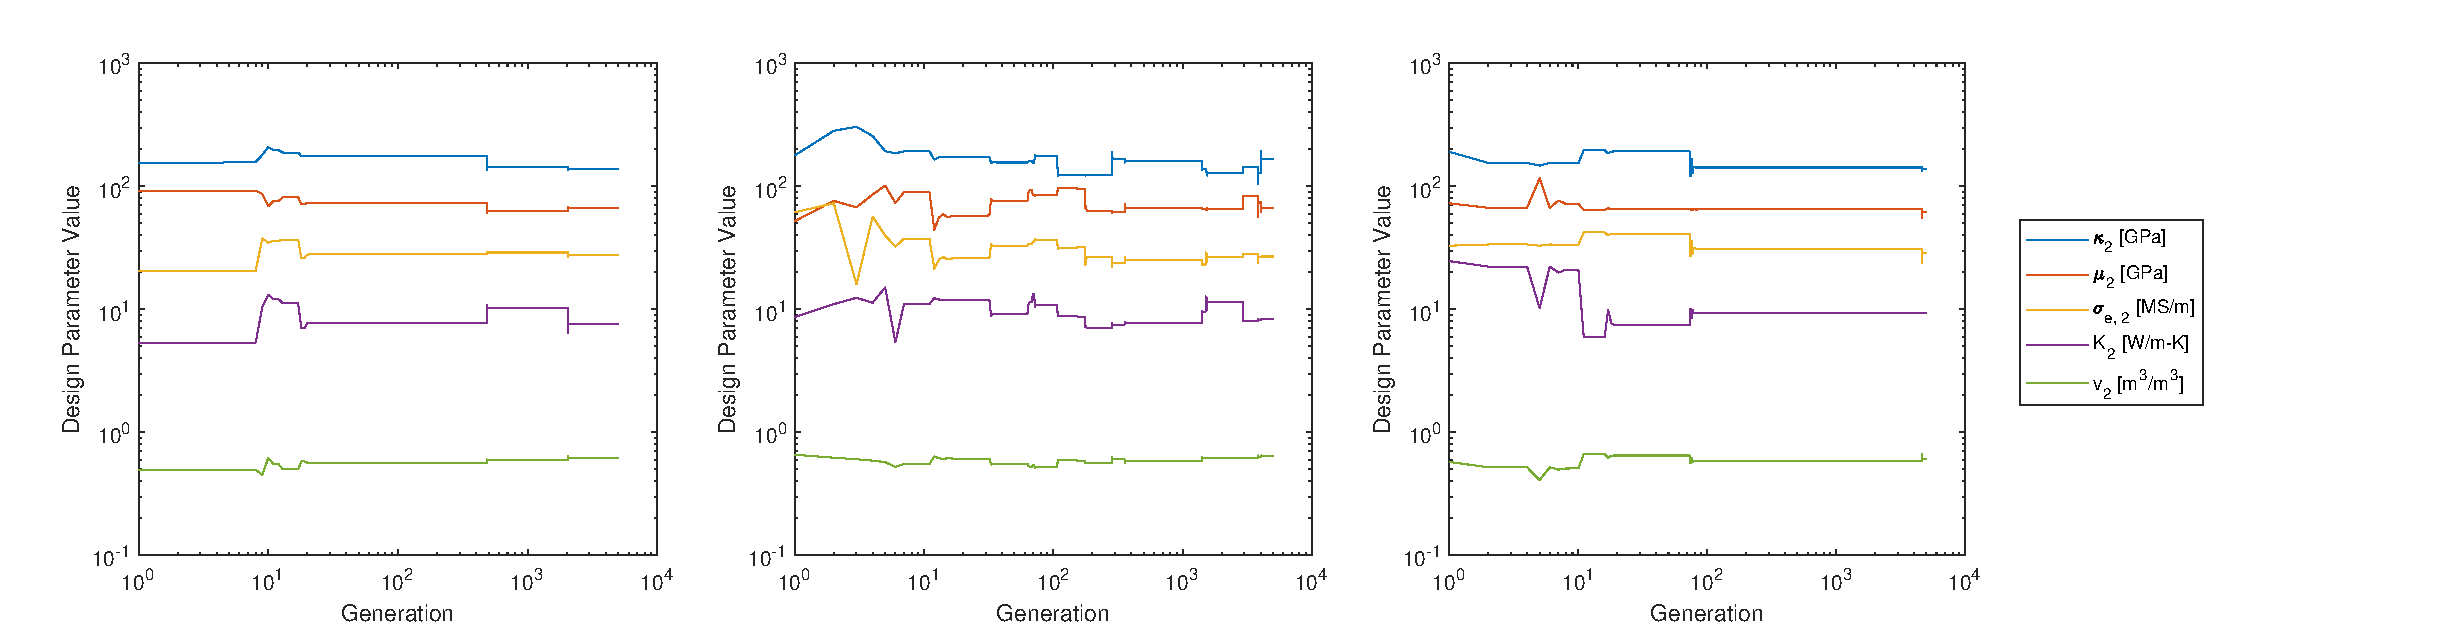
\includegraphics[width=1.2\linewidth]{3-1.eps}
  \caption{Design parameter value of best design vs. generation for various GA types. From left to right: ten parents, zero parents, ten parents with child mutations}
  \end{nscenter}
\end{figure}

\begin{table}[H]
\centering
\caption{Fractional difference between achieved and desired design parameter for various GA types.}
\resizebox{0.75\textwidth}{!}{
\begin{tabular}{c||c|c|c|c}
 GA Variation & $\kappa_2$ & $\mu_2$ & $\sigma_{e,2}$ & $K_2$ \\ 
 \hline
 \hline
Ten Parents & -0.249 & -0.419 & -0.375 & -0.223 \\
Zero Parents & -0.511 & -0.417 & -0.345 & -0.335 \\
Ten Parents, Child Mutations & -0.252 & -0.313 & -0.439 & -0.512 \\
\end{tabular}
}
\end{table}

\begin{table}[H]
\centering
\caption{Sum of absolute fractional differences for various GA types.}
\resizebox{0.75\textwidth}{!}{
\begin{tabular}{c||c}
 GA Variation & Sum of Frational Differences  \\ 
 \hline
 \hline
Ten Parents & 1.266 \\ 
Zero Parents & 1.607 \\ 
Ten Parents, Child Mutations & 1.516 \\
\end{tabular}
}
\end{table}

\begin{table}[H]
\centering
\caption{Best four design strings for GA with ten parents.}
\resizebox{0.75\textwidth}{!}{
\begin{tabular}{c||c|c|c|c|c|c|c}
 Design & $\kappa_2$ & $\mu_2$ & $\sigma_{e,2}$ & $K_2$ & $v_2$ & $\nu$ & $E^y$ \\ 
 \hline
 \hline
1 & 138.651 & 66.708 & 27.504 & 7.581 & 0.625 & 0.293 & 450.550 \\
2 & 138.651 & 66.708 & 27.504 & 7.581 & 0.625 & 0.293 & 450.550 \\
3 & 138.651 & 66.708 & 27.504 & 7.581 & 0.625 & 0.293 & 450.550 \\
4 & 138.651 & 66.708 & 27.504 & 7.581 & 0.625 & 0.293 & 450.550 \\
\end{tabular}
}
\end{table}

\begin{table}[H]
\centering
\caption{Best four design strings for GA with zero parents.}
\resizebox{0.75\textwidth}{!}{
\begin{tabular}{c||c|c|c|c|c|c|c}
 Design & $\kappa_2$ & $\mu_2$ & $\sigma_{e,2}$ & $K_2$ & $v_2$ & $\nu$ & $E^y$ \\ 
 \hline
 \hline
1 & 167.687 & 66.585 & 26.892 & 8.279 & 0.644 & 0.325 & 551.208 \\
2 & 167.687 & 66.585 & 26.892 & 8.279 & 0.644 & 0.325 & 551.208 \\
3 & 167.687 & 66.585 & 26.892 & 8.279 & 0.644 & 0.325 & 551.208 \\
4 & 167.687 & 66.585 & 26.892 & 8.279 & 0.644 & 0.325 & 551.208 \\
\end{tabular}
}
\end{table}

\begin{table}[H]
\centering
\caption{Best four design strings for GA with ten parents and child mutations.}
\resizebox{0.75\textwidth}{!}{
\begin{tabular}{c||c|c|c|c|c|c|c}
 Design & $\kappa_2$ & $\mu_2$ & $\sigma_{e,2}$ & $K_2$ & $v_2$ & $\nu$ & $E^y$ \\ 
 \hline
 \hline
1 & 138.982 & 61.697 & 28.771 & 9.377 & 0.613 & 0.307 & 448.375 \\
2 & 138.982 & 61.697 & 28.771 & 9.377 & 0.613 & 0.307 & 448.375 \\
3 & 138.982 & 61.697 & 28.771 & 9.377 & 0.613 & 0.307 & 448.375 \\
4 & 138.982 & 61.697 & 28.771 & 9.377 & 0.613 & 0.307 & 448.375 \\
\end{tabular}
}
\end{table}


\section{Conclusion}



\section{Appendix}
Appendix is empty.



\end{document}